\section{Auswertung}
\label{sec:Auswertung}

\subsection{Reflektion}
  Für die Reflektion wurden für die Einfallswinkel $\alpha_1$ folgende Ausfallswinkel (in Grad)
  gemessen:
  \begin{table}[H]
    \centering
    \caption{Werte der Reflektion}
    \begin{tabular}{c c}
      \toprule
      $\alpha_1$ & $\alpha_2$\\
      \midrule
        20 & 20.5\\
        30 & 31\\
        40 & 41\\
        45 & 46\\
        50.5 & 51\\
        60 & 60.5\\
        70 & 71\\
      \bottomrule
    \end{tabular}
  \end{table}
  \noindent Diese wurden in der nachfolgenden Grafik geplottet und ihre Steigung $m=1.001 \pm 0.007$
  mittels linearer Regression bestimmt.
  \begin{figure}[H]
    \centering
    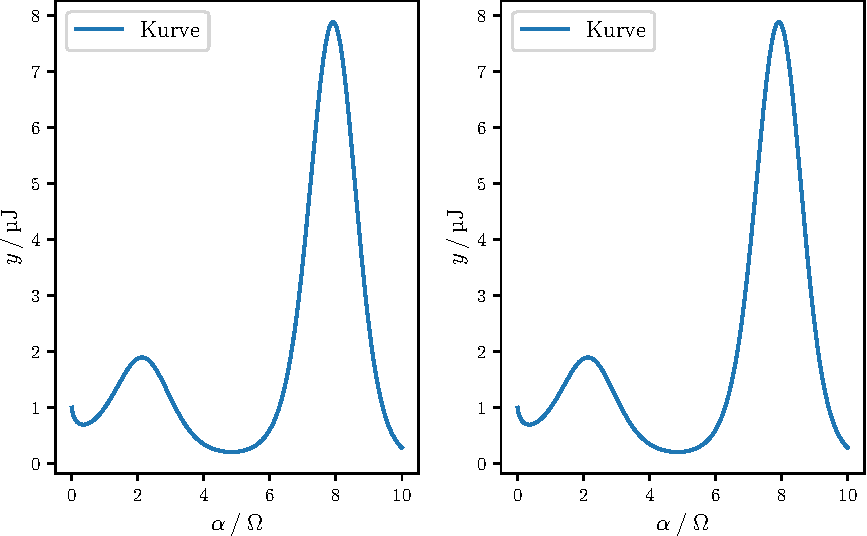
\includegraphics{plot.pdf}
    \caption{Messwerte der Reflektion}
    \label{fig:plot}
  \end{figure}

\subsection{Transmission}
  Folgende Brechungswinkel $\beta$ ergab der zweite Versuch zu den Einfallswinkeln $\alpha$:
  \begin{table}[H]
    \centering
    \caption{Werte der Transmission}
    \begin{tabular}{c c}
      \toprule
      $\alpha$ & $\beta$\\
      \midrule
        10 & 7.25 \\
        20 & 13.5 \\
        30 & 20   \\
        40 & 26   \\
        50 & 31.5 \\
        60 & 36   \\
        70 & 39.5 \\
      \bottomrule
    \end{tabular}
  \end{table}
  \noindent Daraus lassen sich anhand der Formel $n = \dfrac{\sin{\alpha}}{sin{\beta}}$ folgende
  Werte für den Brechungsindex n berechnen:
  \begin{table}[H]
    \centering
    \caption{Brechungsindizes}
    \begin{tabular}{c c}
      \toprule
      $n$\\
      \midrule
        7.25 \\
        13.5 \\
        20   \\
        26   \\
        31.5 \\
        36   \\
        39.5 \\
      \bottomrule
    \end{tabular}
  \end{table}
  \noindent Mittels Numpy wurde daraus der Mittelwert $n=1.53\pm 0.04$ beestimmt. Anhand 
  dieses Wertes wurde die Lichtgeschwindigkeit in dem Glas zu $c_G=\dfrac{c}{n}= (1.95\pm 0.05)
  \cdot 10^{8}$ m/s berechnet.

\subsection{Strahlversatz}
  Für diesen Abschnitt wurden dieselben Werte verwendet, die bereits für den Abschnitt 
  Transmission verwendet wurden.
  Mit der in der Theorie hergeleiteten Formel 
  \begin{equation*}
    s= d\dfrac{\sin{\alpha - \beta}}{cos{\beta}} 
  \end{equation*}
  wird nun der Strahversatz berechnet. Dabei wird zunächst mit den realen Beta-Werten und dann
  mit idealisierten, die durch $\beta=\arcsin{\dfrac{\sin{\alpha}}{n}}$ wurden. Dabei ergeben 
  sich für Beta folgende Werte:

  \begin{table}[H]
    \centering
    \caption{Strahlversatz}
    \begin{tabular}{c c }
      \toprule
      reale $\Beta$-Werte [rad] &  idealisierte $\Beta$-Werte [rad]\\
      \midrule
        0.14 & 0.51 \\
        0.33 & 1.01 \\
        0.51 & 1.51   \\
        0.73 & 2.00   \\
        0.98 & 2.46 \\
        1.28 & 2.91   \\
        1.63 & 3.34 \\
      \bottomrule
    \end{tabular}
  \end{table}
  \noindent Für den Strahlversatz lassen sich die Werte also zu
  \begin{table}[H]
    \centering
    \caption{Strahlversatz}
    \begin{tabular}{c c }
      \toprule
      Strahlversatz mit realen $\Beta$-Werten x $10^{-2}$ & Strahlversatz mit idealisierten $\Beta$-Werten x $10^{-2}$\\
      \midrule
        0.14 & 0.51 \\
        0.33 & 1.01 \\
        0.51 & 1.51   \\
        0.73 & 2.00   \\
        0.98 & 2.46 \\
        1.28 & 2.91   \\
        1.63 & 3.34 \\
      \bottomrule
    \end{tabular}
  \end{table}
  berechnen.

\subsection{Prisma}
  Nun wird die Brechhung von Licht unterschiedlicher Wellenlänge in einem Prisma betrachtet.
  Verwendet werden ein grüner und ein roter Laser. 